\chapter{执行纲要}

\section{市场描述}
亲子互动是指家庭中父母与子女之间的互动。这是一种增进儿童与父母和其他
家庭成员之间感情,加强家庭凝聚力,培养儿童归属感和父母责任感的有益方式。
随着市场经济的不断发展,人们的对精神层面的需求日益增加。
在国外,很多餐馆都推出了亲子套餐,许多娱乐节目也推出了亲子活动。例如,《爸爸
去哪儿》系列显示此列活动非常受欢迎。

从家庭活动的角度来看,就餐是父母与孩子沟通的重要时刻。然而,许多父母忙于工作,经常
不能和孩子一起用餐,对孩子的培养造成了损失。另外,即使父母和孩子一起
用餐,然而餐厅的气氛也往往不适合家人之间的沟通,家人出去吃饭却无话可说的尴尬局面也是
一个普遍的现象。父母和孩子需要一个环境与家庭相似的餐厅,每个家庭都可以有一个
相对独立的环境,餐馆配备了各种亲子互动设施,在这里,父母和孩子不但可以享受美食,
还可以共享天伦之乐。

目前,这种在中国的亲子主题餐厅很少,这意味着这个市场是一片蓝海;而亲子互
动中潜在的巨大商机足以说服投资者。国家实施全面二孩政策。从长远来看,人口已进
入增长期。二胎宝宝成为一个巨大的市场。独生子女家庭的数量减少,第二胎家庭数量
增加:家庭结构发生了变化。家长需要花更多的时间与孩子在一起。随着中国大学及以
上人口比例的增加,家长的素质不断提高,这意味着父母对孩子的投资会相应增加。亲
子餐厅与时代潮流保持一致,为家长和孩子提供一个餐饮,娱乐和情感交流的场所。

根据市场调查,中国的亲子餐厅很少,北京,上海和广州只有一家餐厅。这表明中
国的亲子餐饮市场还没有形成大公司的垄断。此外,随着人们对子女的投资力度不断加
大,对子女的精神需求越来越重视,对亲子餐厅的市场需求远未饱和。

\begin{figure}[ htbp ]
        \centering
        \caption{我国近两年出生人口}
        % This is a minimal histogram using ``pgfplots''.
% There is still a huge space to tune it.

\begin{tikzpicture}
        \begin{axis}[
                        % Make the bar wider
                        bar width=20pt,
                        % Give x symbolic names
                        symbolic x coords={十二五时期, 2016, 2017},
                        % Generate labels below axies
                        xlabel={ 年份 },
                        ylabel={ 人口 },
                        xtick=data
                ]
                \addplot[ybar, fill=blue] coordinates {
                        % For tiny datasets, list them as coordinates
                        (十二五时期,1644)
                        (2016,1786)
                        (2017,1723)
                };
        \end{axis}
\end{tikzpicture}

\end{figure}
\begin{figure}[ htbp ]
        \centering
        \caption{市场份额}
        \label{figure:market-share}
        % This Pie Chart uses the ``pgf-pie'' package which is based on pgfplots
% and **not** hosted on CTAN but mirrored on Github (cause Google Code shutdown).
% Although people on StackExchage vote against using this package or even using
% Pie Chart, we used it here to get close look and feel as with the one produced
% by WYSIWYG WPS.

% This package is the first one installed manually by me. I learnt the TDS (TeX Dir Struct)
% from here and dropped .sty and pdf manual to the right places under $TEXMFHOME and run
% texhash and I could use it like ``\usepackage{pgf-pie}'' and view its doc by ``texdoc pgf-pie''.

\begin{tikzpicture}
        % Legend means small colorful tags telling the identity of each colorred object
        \pie[text = legend]{
                30/广州熊猫餐厅,
                40/北京麦幼优儿童主题餐厅,
                30/上海芭迪熊儿童主题餐厅
        }
\end{tikzpicture}

\end{figure}
\begin{figure}[ htbp ]
        \centering
        \caption{某家亲子餐厅内景}
        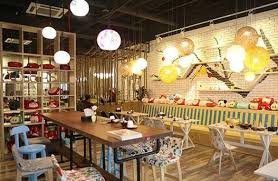
\includegraphics{../images/interior/内景1}
\end{figure}
\begin{figure}[ htbp ]
        \centering
        \caption{另一家亲子餐厅内景}
        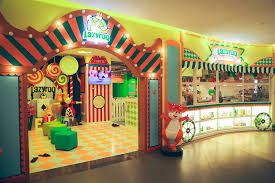
\includegraphics{../images/interior/内景2}
\end{figure}

\section{核心技术}
作为一家餐馆,食品的供应是最重要的技术之一。作为一家亲子主题餐馆,我们有
专业的装潢师、会做各式家常菜的厨师、布景师等等。为了能够提供更好的服务,我们
还有表演团队为家庭庆典提供庆祝演出。本项目的特色主要有:特色童餐、主题装潢、
亲子活动和特色自助餐。

\begin{description}
\item[特色童餐:] 餐厅的特色菜品为儿童餐,兼顾了美味、健康和新颖。提供适合儿童好
奇心理的和照顾了儿童消化系统的菜品,以精美、色彩斑斓和营养均衡为特色。

\item[主题装潢:] 在装修上走类似迪士尼乐园的故事主题装修路线,有适合不同年龄段儿
童,从童话故事,小说,电影中提取的经典场景,如星球大战主题;冰河主题;小黄人
主题等。

\item[亲子活动:] 提供丰富多彩的亲子活动,包括户内的蛋糕 DIY、亲子陶艺、英语沙龙
等项目和户外的亲子拔河、两人三足、亲子吹乒乓球等项目。利用用餐前后或者节假日
等时段开展。其中户外活动和餐饮联动,参加户外活动的顾客可以获得就餐优惠。此外
还承接各种节日派对。

\item[特色自助餐:] 除此之外,餐厅还提供品种丰富、精选各国特色美食的自助餐,为不
同顾客提供了不同的选择。
\end{description}

\section{团队概述}
% 我们团队只有我一个人,我只懂排版,其他两个队友是我凑来的:(
我们的团队最初的成员是来自北航餐饮厨艺协会的三位会员。随着我们创业计划的
推广,越来越多不同院系的同学加入了我们。目前,我们有来着计算机系的负责开发手
机 APP 点餐系统、网页开发等等 IT 业务的同学;有来着法学院的负责法律顾问的同学;
由来着经管学院的负责财务的同学;还有来着北京农业大学的同学,负责采购原材料。
还有从社会招募来的服务员和演员。

团队核心成员共 20 名,分工明确,主要负责餐馆的日常经营,菜式的研发,亲子
活动的策划以及线上推广。团队已经开发了完整的运作流程,进行了详尽的市场分析,
撰写了完善的商业项目策划,目前已经完成了创业前期的大部分工作。

\section{发展战略}
\begin{description}
\item [ 近期发展目标(1-2 年):] 在北京经营 3-4 家分店,积累活跃顾客,建立“亲子
互动”,“亲子共享美食”的新的生活风尚。加大宣传力度,开发点餐 APP。在“饿了吗”等
外卖平台提供服务、在微信建立公众号、在微博建立官微、在大众点评获得比较好的评
价等等。

\item [ 中期发展目标(3-5 年):]  把分店扩散到其他省份,特别是餐饮消费占百分比
较高的省份。开始走中高档路线,提高服务质量,提供更多增值服务,比如亲子卡拉
OK,亲子脱口秀,生日送蛋糕等等。

\item [ 长期发展目标(5-10 年):]  提升品牌知名度,打造国内亲子主题餐饮领先品牌,
开发国外市场,提供国际化的亲子主题餐饮服务。
\end{description}
